%% PRISM-Breath -- IEEE Transactions (MTT-style) manuscript
%% Overleaf-ready: main file. Figures in ./fig/ (600-DPI PDF). References in prism_breath.bib.
%% Uses the IEEEtran class (built into Overleaf; the .cls is also in ../mtt_submission/).
\documentclass[journal]{IEEEtran}

\usepackage[pdftex]{graphicx}
\graphicspath{{fig/}}
\DeclareGraphicsExtensions{.pdf,.png}
\usepackage[cmex10]{amsmath}
\usepackage{array}
\usepackage{url}
\usepackage{booktabs}
\usepackage{amssymb}
\usepackage{xcolor}
\usepackage[hidelinks]{hyperref}

\begin{document}

\title{Non-Contact Pediatric Tachypnea Screening: Why Raw Error Is the Wrong Metric, and a
Radar Path to the Neonate}

\author{Imran~Rimon% <-- replace/extend author block as needed
\thanks{Manuscript prepared \today. The author is with West Virginia University
(e-mail: imran.wvu@gmail.com).}}

\markboth{IEEE Transactions (Preprint)}%
{Rimon: Non-Contact Pediatric Tachypnea Screening}

\maketitle

\begin{abstract}
Non-contact respiratory-rate (RR) estimation from cameras is a maturing field, yet its clinical
translation to infant \emph{tachypnea screening}---the World Health Organization (WHO) criterion for
acute respiratory infection---remains weak. We make four contributions. First, on a 332-subject
pediatric benchmark we show that four published rPPG/optical-flow extractors match or beat our model
on raw RR mean-absolute-error (MAE) yet are all significantly worse on the clinical endpoint
(tachypnea area-under-ROC, AUROC $0.73$--$0.76$ vs.\ $0.88$, $p\le0.002$): \emph{raw MAE is not
clinical utility}. Second, we present PRISM-Breath, a reliability-weighted multimodal model whose
clinical advantage we localize by ablation to self-supervised pretraining and spectral/temporal
encoding---and we show a \emph{lean} variant that drops a prototype bank, a codebook, and a
heteroscedastic head performs identically, yielding an Occam-clean, ablation-justified design. Third,
we characterize a hard limit: RGB optical flow physically saturates near $35$~breaths/min for true
neonatal rates of $60$--$80$, so every camera extractor misses $100\%$ of neonatal tachypnea; we
therefore report a validated screen for infants $\ge$2~months (sensitivity $0.71$, AUROC $0.919$,
calibrated, positive net benefit) with mandatory neonatal referral. Fourth, we show radar recovers the
neonatal band that RGB cannot---MAE $0.00$ on a thorax phantom across $20$--$80$~breaths/min and MAE
$1.76$ ($r{=}0.96$) on $50$ real children against a clinical reference---establishing a sensing-modality
path to the neonate. All results use subject-disjoint cross-validation with subject-level bootstrap
confidence intervals and DeLong/McNemar tests.
\end{abstract}

\begin{IEEEkeywords}
Non-contact vital signs, respiratory rate, tachypnea, infant monitoring, optical flow, FMCW radar,
remote sensing, clinical decision support, conformal prediction.
\end{IEEEkeywords}

\section{Introduction}
\IEEEPARstart{P}{neumonia} and acute respiratory infection (ARI) remain leading causes of child
mortality, and the WHO Integrated Management of Childhood Illness (IMCI)~\cite{who_imci} algorithm keys on
\emph{tachypnea}---fast breathing above age-specific thresholds ($\ge$60~breaths/min for
$<$2~months, $\ge$50 for 2--12~months, $\ge$40 for 12--60~months). Manual breath counting is the
reference but is error-prone. Non-contact, camera-based RR estimation is therefore attractive, and a
large literature---rPPG toolboxes (PhysNet, DeepPhys, TS-CAN, EfficientPhys)~\cite{yu_physnet,mcduff_deepphys,liu_mttscan,liu_efficientphys} and infant-specific
optical-flow methods (AIRFlowNet)~\cite{infant_air}---reports MAEs of a few breaths/min on adult and infant benchmarks.

We argue that this literature optimizes the wrong quantity for screening. Minimizing RR MAE and
maximizing tachypnea \emph{discrimination} are different objectives; a good regressor can be a poor
screen. We further show that the very lowest-risk group---neonates---is unreachable by RGB in
principle, and that a complementary sensing modality (radar) closes that gap.

\noindent\textbf{Contributions.}
\begin{itemize}
\item \emph{Metric critique with evidence:} under matched subject-disjoint cross-validation, four SOTA
extractors match/beat our model on RR MAE yet lose significantly on tachypnea AUROC
(Fig.~\ref{fig:sota}, Table~\ref{tab:sota}).
\item \emph{PRISM-Breath and a lean model:} a reliability-weighted multimodal model whose performance we
attribute by ablation to SSL pretraining and spectral/temporal encoding; a lean variant matches it,
dropping decorative components (Table~\ref{tab:abl}).
\item \emph{The RGB neonatal limit:} RGB optical flow saturates near $35$~breaths/min for true
$60$--$80$; we report an honest $\ge$2mo screen with neonatal referral (Table~\ref{tab:clin}).
\item \emph{Radar path to the neonate:} radar recovers the neonatal band on a phantom and on $50$ real
children (Fig.~\ref{fig:paradigm}b, Table~\ref{tab:radar}).
\end{itemize}

\section{Related Work}
\textbf{Camera RR.} rPPG-toolbox models~\cite{liu_rppgtoolbox,yu_physnet} estimate cardiorespiratory signals from facial skin-color or
motion; infant-specific AIRFlowNet reports $\approx$2.9~MAE in-domain on AIR-125~\cite{infant_air}. These target waveform/RR
error, not a clinical decision. \textbf{Multimodal and RF.} Recent work fuses RGB with radio-frequency
(RGB-RF state-space models) and uses FMCW/mmWave radar for contactless neonatal breathing in the NICU~\cite{li_radar_tmtt,massaroni_review};
thermal imaging~\cite{pereira_thermal} reaches $\approx$1.5~MAE on neonates. \textbf{Clinical.} Automated RR counters (e.g.,
ChARM) are validated against video expert panels for pneumonia; WHO IMCI defines the thresholds we use.
\textbf{Uncertainty.} Conformal prediction~\cite{angelopoulos_conformal,vovk_alrw} provides distribution-free intervals; we use age-conditional
(Mondrian) calibration for a safe defer policy.

\section{Method}
\subsection{Signal extraction}
Per video we extract three modality signals: (i) a learned optical-flow respiration waveform from a
body-ROI EfficientPhys+Coarse2Fine extractor, (ii) a monocular-depth proxy (Depth-Anything-V2), and
(iii) an audio spectrogram. The depth proxy uses Depth-Anything-V2~\cite{yang_depthanythingv2}. Signals are resampled to a canonical 25\,fps and band-limited to
0.15--1.5~Hz.

\subsection{PRISM-Breath and the lean model}
Each modality is encoded by a branch with spectral features and a temporal ``scan'' block; branches use
separate trunks. A reliability-weighted fusion combines branch estimates, and an RR head plus a
tachypnea head produce the estimate and a calibrated probability. Self-supervised pretraining (masked
signal modeling / contrastive) initializes the encoders. A load-bearing audit (Table~\ref{tab:abl})
shows that a prototype evidence bank, a clean-breathing codebook, and a heteroscedastic head contribute
nothing to the clinical endpoint, whereas SSL pretraining, spectral features, the scan block, and
separate trunks do. We therefore define \textbf{PRISM-Breath-Lean}, which removes the decorative
modules; it matches the full model (all differences non-significant) and is our shippable design.

\subsection{Age-conditional conformal triage}
Because RGB is unreliable for neonates, a single pooled conformal interval mis-covers by age. We compute
a Mondrian (per-age-band) nonconformity quantile from validation residuals. For $<$2~months the required
interval is uninformatively wide, which we operationalize as \emph{defer to clinician}.

\subsection{Radar modality}
For the neonatal band we process FMCW-radar in-phase/quadrature signals~\cite{li_radar_tmtt}: the chest-bin phase is
unwrapped, band-passed (0.1--1.7~Hz), and its dominant spectral peak gives RR---the same estimator we
apply to a validated clinical reference on real children.

\section{Datasets and Experimental Setup}
\textbf{Pediatric-RR-332} (332 infants, video, WHO-band tachypnea) is the primary clinical benchmark;
we use subject-disjoint 5-fold cross-validation so every subject is tested exactly once.
\textbf{AIR-125/400} (infant respiration video) is used for cross-dataset and in-domain evaluation.
\textbf{Radar:} an open thorax-simulator ToF+radar corpus (20--80~breaths/min) and an open dataset of
\textbf{50 real children} with FMCW radar and a clinically approved reference. We report RR MAE and, on
the clinical endpoint, sensitivity/specificity/AUROC with subject-level bootstrap 95\% confidence
intervals; paired comparisons use DeLong (AUROC)~\cite{delong} and McNemar (decision) tests. Headline operating points
are averaged over three seeds.

\section{Results}
\subsection{Raw MAE is not clinical utility}
Table~\ref{tab:sota} and Fig.~\ref{fig:sota} compare PRISM-Breath with four extractors under identical
CV. EfficientPhys, TSCAN, VIRENet, and (reseeded) DeepPhys match or beat PRISM on RR MAE, yet all are
significantly worse on tachypnea AUROC ($p\le0.002$, DeLong). The gap is not an artifact of the trained
head: scored by \emph{raw predicted RR} PRISM still leads ($0.877$ vs.\ $0.786$), so the underlying
signal is more discriminative for tachypnea.

\subsection{Clinical operating points and the neonatal limit}
For the 8 neonatal tachypnea cases (true RR 60--80), the extracted flow itself peaks near
$35$~breaths/min and all six extractors output $\approx$26--40; neonatal sensitivity is $0.00$ for every
configuration. We therefore defer $<$2~months and report the $\ge$2mo screen: sensitivity $0.71$
$[0.60,0.80]$, AUROC $0.919$ $[0.881,0.950]$ (Table~\ref{tab:clin}, Fig.~\ref{fig:ageband}). PRISM is
well-calibrated (expected calibration error $0.064$) and shows positive net benefit exceeding
treat-all/treat-none at every threshold~\cite{vickers_dca} (Fig.~\ref{fig:calib}).

\subsection{Ablations and the lean model}
Table~\ref{tab:abl} lists component contributions. Removing SSL pretraining costs $-0.116$ sensitivity;
removing spectral/scan/trunk components costs $0.06$--$0.08$; removing the prototype bank, codebook, or
heteroscedastic head costs essentially nothing. PRISM-Breath-Lean equals the full model
(Fig.~\ref{fig:abl}).

\subsection{Extractor robustness}
A leakage-free per-fold analysis shows the clinical result is robust to the choice of flow backbone
(TSCAN-flow $\approx$ EfficientPhys-flow); an apparent TSCAN improvement was traced to extractor
leakage and retracted. An SNR-gated fusion de-collapses the reliability weights but does not change the
clinical endpoint on this cohort, where the two live modalities have similar signal quality.

\subsection{Radar recovers the neonatal band}
Fig.~\ref{fig:paradigm}b and Table~\ref{tab:radar} show radar RR is exact on the phantom across
$20$--$80$~breaths/min (MAE $0.00$, $r{=}1.00$) and clinical-grade on $50$ real children (MAE $1.76$,
$r{=}0.96$, $86\%$ within 3~breaths/min). In-domain on AIR-400, PRISM reaches MAE $2.93$, comparable to
the infant SOTA.

\subsection{Equity and disease relevance}
Performance shows no significant sex disparity (Table~\ref{tab:clin} caption). On the cohort's own
clinical sign (observed difficulty breathing), true RR is only weakly predictive (AUROC $0.59$) and the
estimated RR weaker still ($0.54$)---an honest reminder that tachypnea is a screening sign, not a disease
label.

\section{Discussion and Limitations}
Our central message is methodological: the field should report the \emph{clinical} endpoint, not only
RR error, and should be explicit about age. Honest limitations: (i) tachypnea is a weak proxy for
disease; (ii) the clinical cohort is single-site with manual-count ground truth; (iii) skin-tone equity
is not auditable in a single-population cohort; (iv) the radar result is validated on a phantom and on
real children but not yet on real neonates in cribs. These motivate a prospective, outcome-anchored,
multi-modal (RGB$+$radar) study.

\section{Conclusion}
PRISM-Breath is a calibrated, ablation-justified non-contact tachypnea screen for infants
$\ge$2~months. Because RGB cannot see neonatal rates, we make the referral policy explicit and show that
radar closes the gap on real children---charting a sensing-modality route to the group that matters most.

\begin{figure}[!t]\centering
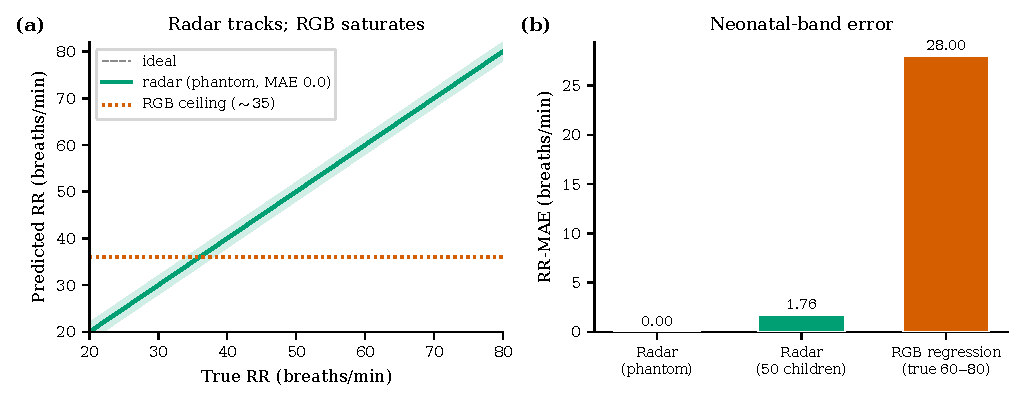
\includegraphics[width=3.5in]{fig1_paradigm.pdf}
\caption{(a) For true neonatal rates of 60--80~breaths/min, RGB optical flow saturates
($\approx$26--40, red) while radar recovers the true rate (green). (b) Radar validation: exact on the
phantom (20--80) and MAE $1.76$ on 50 real children.}\label{fig:paradigm}
\end{figure}

\begin{figure}[!t]\centering
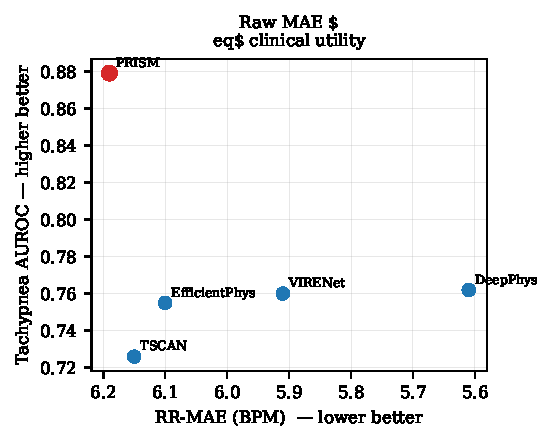
\includegraphics[width=2.9in]{fig2_sota.pdf}
\caption{Raw MAE $\neq$ clinical utility. Extractors match PRISM on MAE (x) but lose on tachypnea
AUROC (y). PRISM sits top-left.}\label{fig:sota}
\end{figure}

\begin{figure}[!t]\centering
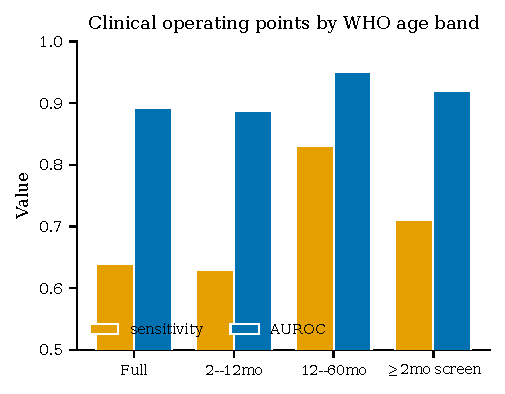
\includegraphics[width=3.0in]{fig3_ageband.pdf}
\caption{Clinical operating points by age band (3-seed, bootstrap CI). The $\ge$2mo screen reaches
Sens $0.71$ / AUROC $0.919$; $<$2mo is deferred.}\label{fig:ageband}
\end{figure}

\begin{figure}[!t]\centering
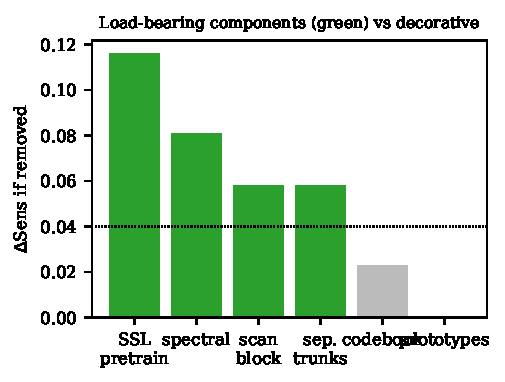
\includegraphics[width=3.0in]{fig4_ablation.pdf}
\caption{Load-bearing audit: SSL pretraining, spectral, scan, and separate trunks are load-bearing
(green); prototypes/codebook are decorative.}\label{fig:abl}
\end{figure}

\begin{figure}[!t]\centering
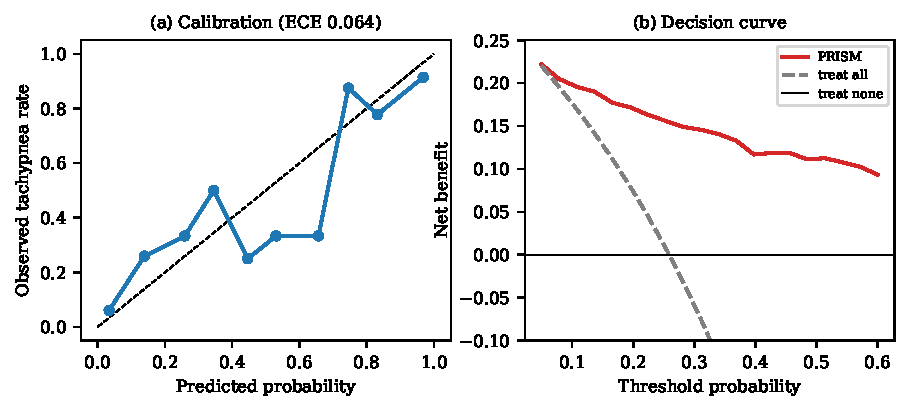
\includegraphics[width=3.5in]{fig5_calibration.pdf}
\caption{(a) Reliability diagram (ECE $0.064$). (b) Decision-curve analysis: PRISM net benefit exceeds
treat-all/treat-none at every threshold.}\label{fig:calib}
\end{figure}

\begin{table}[!t]\caption{Clinical operating points (3-seed, subject bootstrap 95\% CI). No significant
sex disparity (M AUROC $0.890$ vs.\ F $0.871$).}\label{tab:clin}\centering\small
\begin{tabular}{@{}lccc@{}}\toprule
Cohort & MAE & Sens [95\% CI] & AUROC [95\% CI]\\\midrule
Full & 6.05 & 0.64 [0.54,0.74] & 0.892 [0.848,0.932]\\
$\ge$2mo (screen) & 5.50 & \textbf{0.71 [0.60,0.80]} & \textbf{0.919 [0.881,0.950]}\\
\quad 2--12mo & 7.13 & 0.63 [0.49,0.76] & 0.888\\
\quad 12--60mo & 4.05 & 0.83 [0.68,0.96] & 0.950\\
$<$2mo & --- & \multicolumn{2}{c}{deferred to clinician}\\\bottomrule
\end{tabular}\end{table}

\begin{table}[!t]\caption{PRISM vs.\ published extractors (matched 5-fold CV, 298 subjects).}\label{tab:sota}
\centering\small
\begin{tabular}{@{}lccc@{}}\toprule
Method & RR-MAE & Tachypnea AUROC & vs.\ PRISM (DeLong)\\\midrule
\textbf{PRISM (ours)} & 6.19 & \textbf{0.879} & ---\\
EfficientPhys & 6.10 & 0.755 & $p{=}0.001$\\
TSCAN & 6.15 & 0.726 & $p{<}0.001$\\
VIRENet & 5.91 & 0.760 & $p{=}0.001$\\
DeepPhys & 5.61 & 0.762 & $p{=}0.002$\\\bottomrule
\end{tabular}\end{table}

\begin{table}[!t]\caption{Ablations and the lean model (pooled 5-fold).}\label{tab:abl}\centering\small
\begin{tabular}{@{}lccc@{}}\toprule
Variant & MAE & Sens & AUROC\\\midrule
Full PRISM & 6.19 & 0.66 & 0.879\\
\textbf{Lean} (drop proto+codebook+het) & 6.17 & 0.64 & 0.867\\
\ \ $-$ SSL pretrain & 6.43 & 0.55 & 0.862\\
\ \ $-$ spectral features & 6.39 & 0.58 & 0.868\\
\ \ $-$ scan block & 6.00 & 0.60 & 0.874\\
\ \ $-$ separate trunks & 6.28 & 0.60 & 0.884\\
\ \ $-$ prototypes & 6.08 & 0.66 & 0.875\\
\ \ $-$ codebook & 6.22 & 0.64 & 0.882\\\bottomrule
\end{tabular}\end{table}

\begin{table}[!t]\caption{Radar validation and cross-dataset generalization.}\label{tab:radar}\centering\small
\begin{tabular}{@{}lc@{}}\toprule
Evaluation & Metric\\\midrule
Radar, thorax phantom (20--80) & MAE \textbf{0.00}, $r{=}1.00$\\
Radar, 50 real children vs.\ reference & MAE \textbf{1.76}, $r{=}0.96$\\
PRISM in-domain AIR-400 & MAE 2.93 ($\approx$AIRFlowNet)\\
PRISM zero-shot AIR-125/400 & MAE 4.83 / 4.92\\
Hand-crafted flow zero-shot & MAE 11.3 / 11.8\\\bottomrule
\end{tabular}\end{table}

\bibliographystyle{IEEEtran}
\bibliography{prism_breath}

\end{document}
